\newpage
\section{Resultados}

Os resultados foram obtidos para cada circuito.

\subsection{Circuito 1}

Utilizando a eq. \ref{e_ganho}, temos:

\[
G_{teorico} = \frac{10e3+5,6e3}{10e3} = 1,56 \quad \bigg [ \frac{V}{V} \bigg ]
\]

A partir da eq. \ref{e_fc}, encontramos que

\[
f_{c teorico} = \frac{1}{2\pi\sqrt{22e^322e^31.4e^{-9}1.4e^{-9}}} = 5170 \quad [Hz]
\]

Após simular o circuito, foi obtido o gráfico mostrado na figura \ref{f_bode1}.

\begin{figure}[H]
\centering
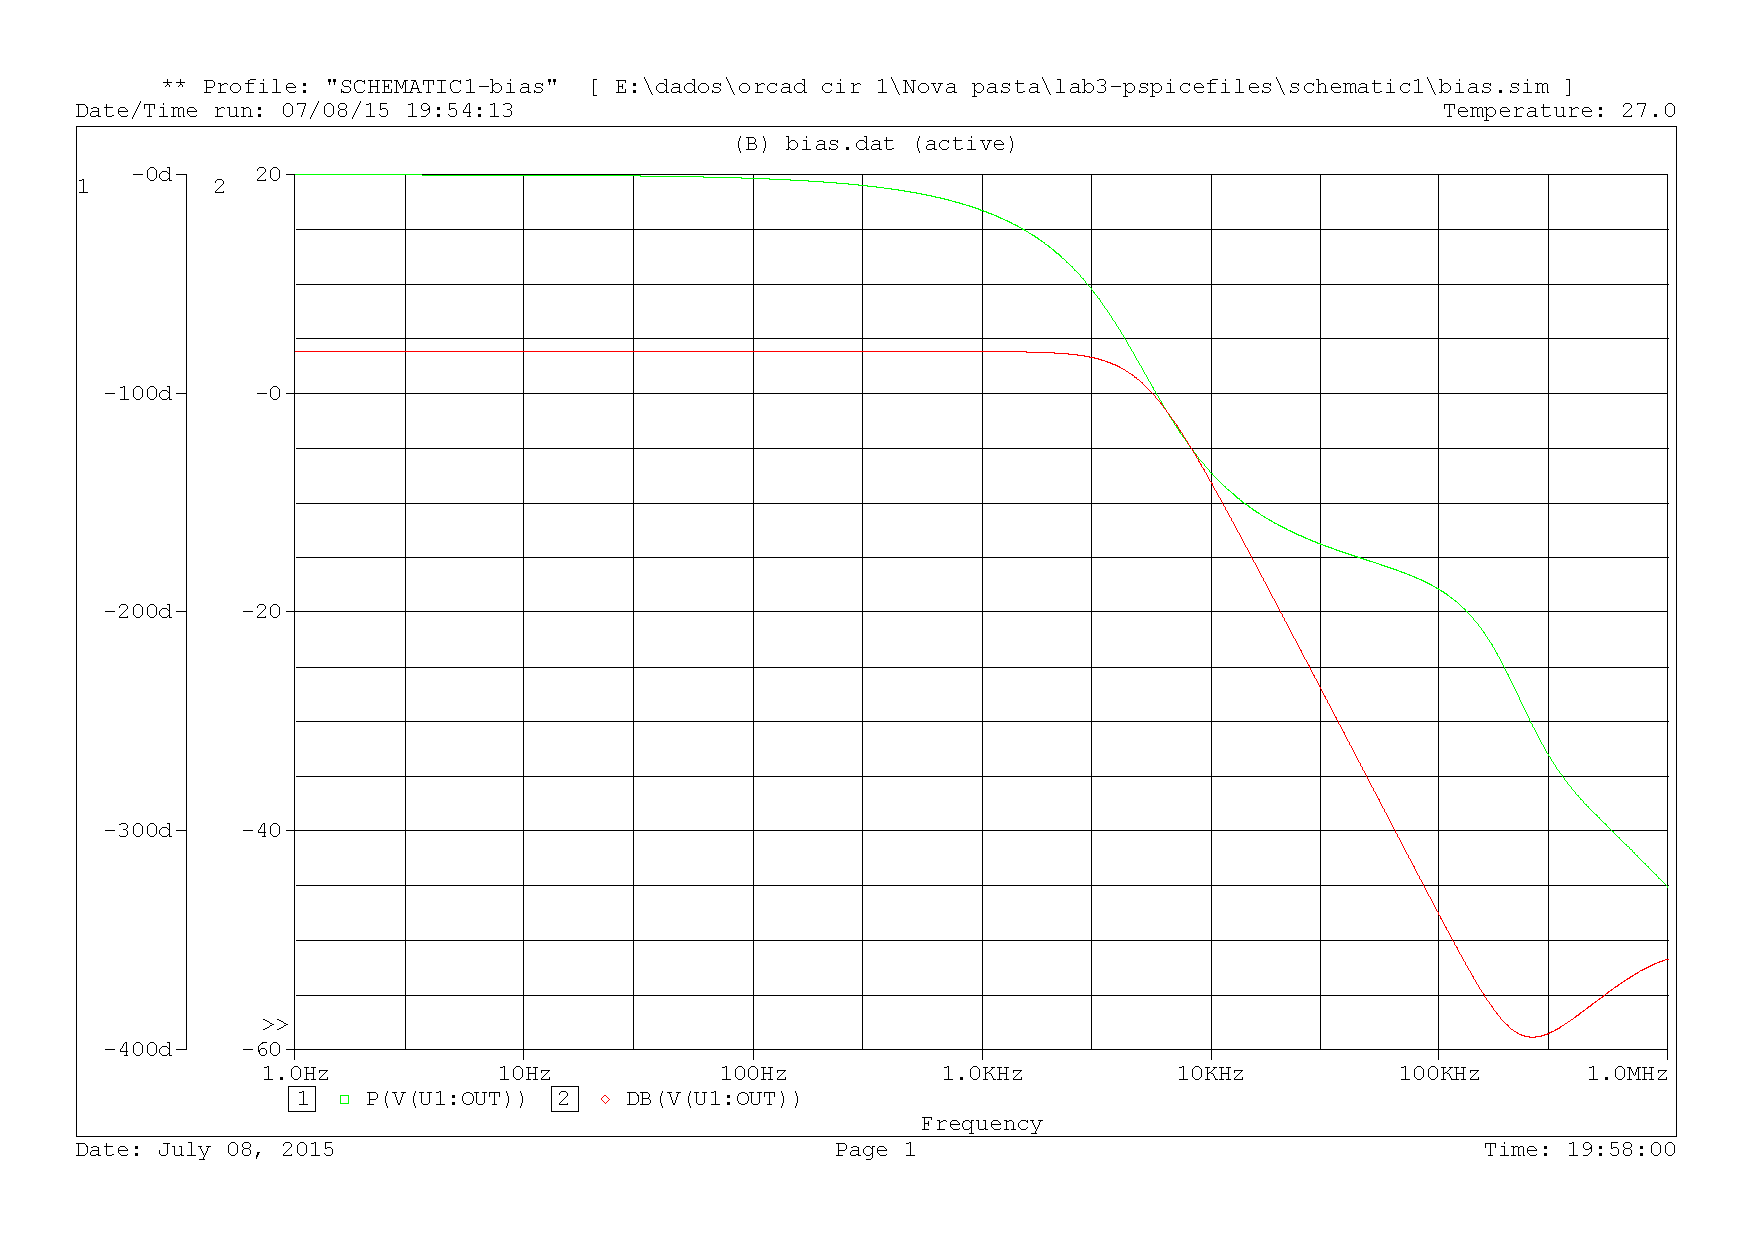
\includegraphics[scale=0.5]{Imagens/bode1.pdf}
\caption{Frequência e fase para o filtro passa-baixas.}
\label{f_bode1}
\end{figure}
  
  A frequência de corte encontrada a partir do gráfico foi $f_c = 5058 \quad [Hz]$ e o ganho $G = 3.862 \quad [dB]$.
  
Como pode ser observado no gráfico da figura \ref{f_bode1}, a atenuação é de -40 dB por década e o tipo de resposta é Butterworth.

\subsection{Citcuito 2}

Para o primeiro estágio, a frequência de corte teórica é $f_{c1} = 4545 \quad [Hz]$ e a frequência de corte simulada é $f_{c1} = 4398 \quad [Hz]$. A figura \ref{f_bode2} mostra o gráfico da resposta em frequência do primeiro estágio. Este filtro é um Chebyshev passa-baixas, com atenuação -38,7 dB/década (segunda ordem) e ganho de -151 [V/V].
Note que o valor do ganho é negativo devido ao amplificador inversor.

\begin{figure}[H]
\centering
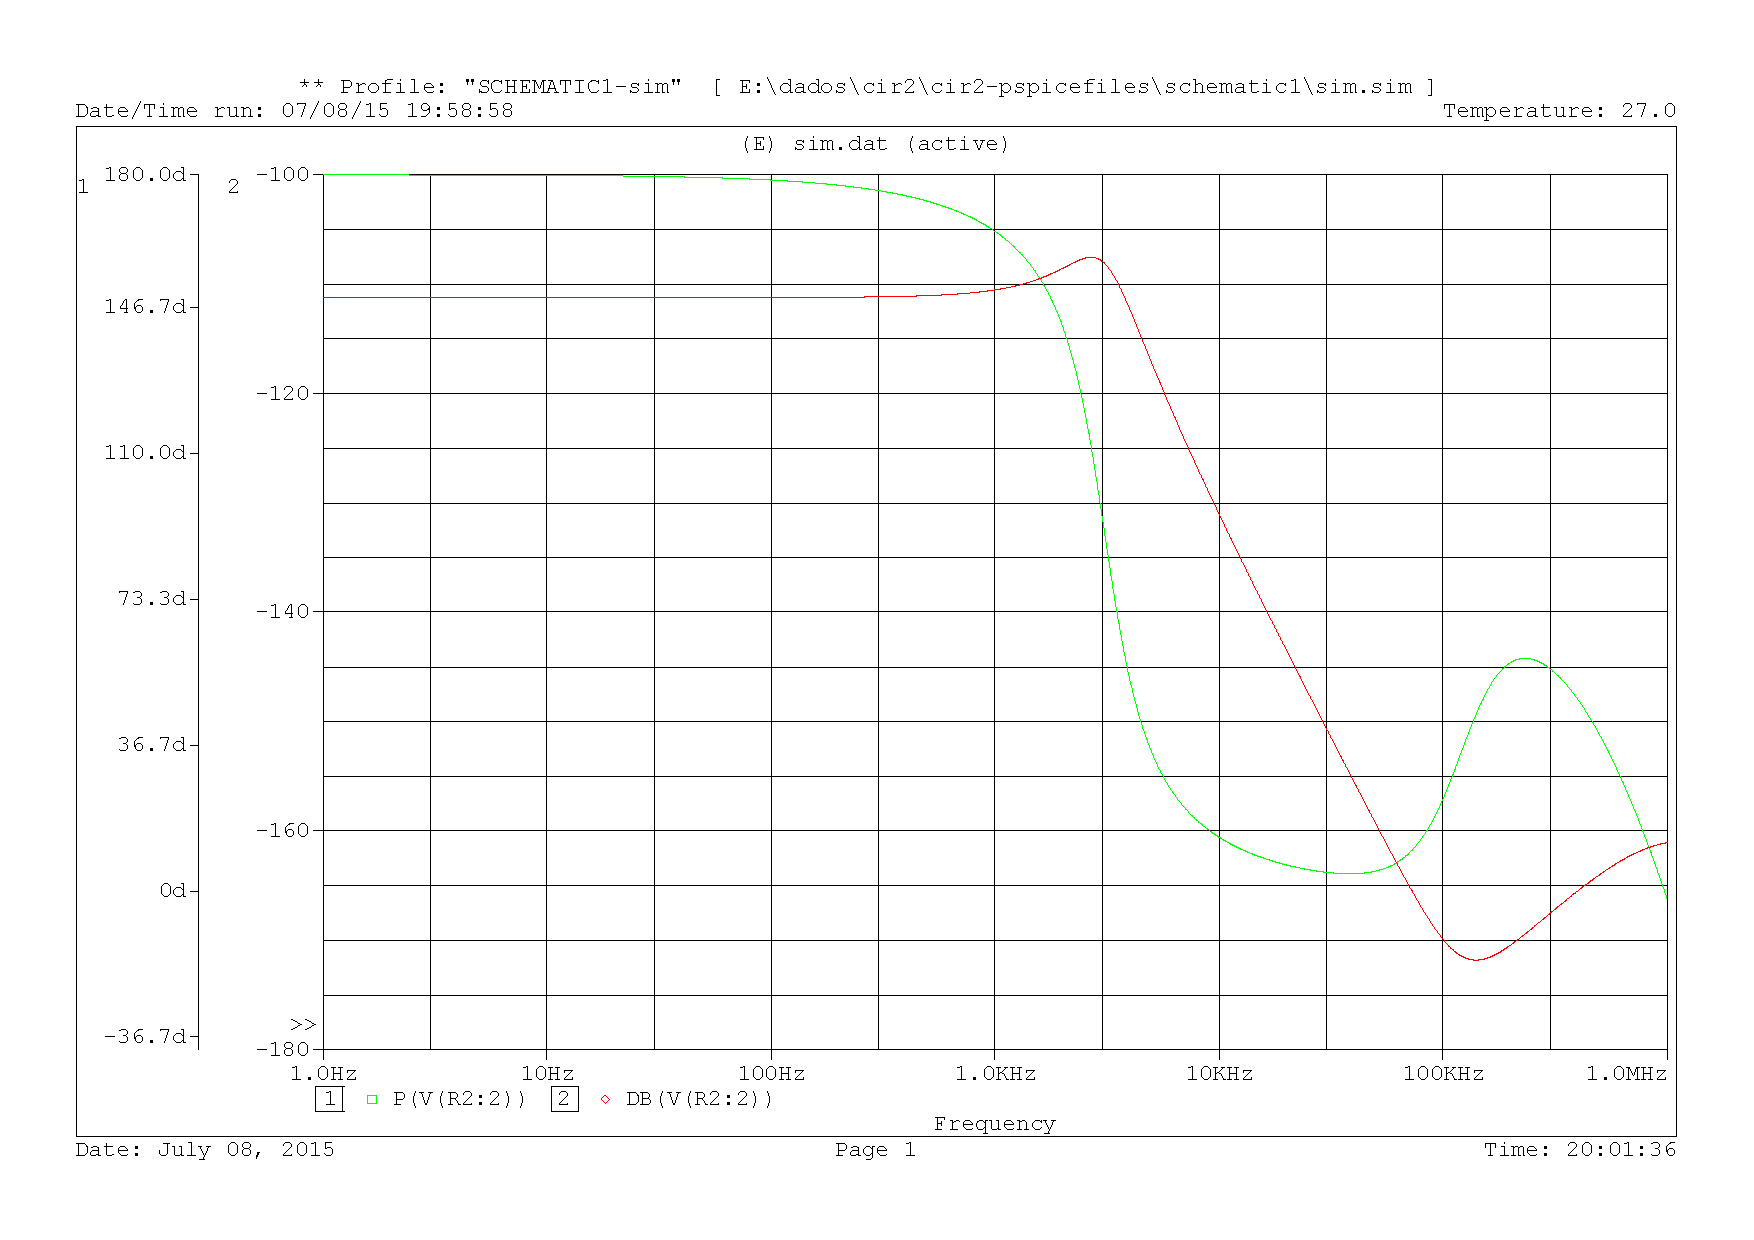
\includegraphics[scale=0.5]{Imagens/bode2.pdf}
\caption{Frequência e fase para primeiro estágio do filtro em cascata.}
\label{f_bode2}
\end{figure}


Para o segundo estágio, a frequência de corte teórica é $f_{c1} = 3150 \quad [Hz]$ e a frequência de corte simulada é $f_{c1} = 3039 \quad [Hz]$. A figura \ref{f_bode3} mostra o gráfico da resposta em frequência do segundo estágio. Este filtro é um passa-baixas, com atenuação -40 dB/década (segunda ordem) e ganho de -154 [V/V].
Note que o valor do ganho é negativo devido ao amplificador inversor.

\begin{figure}[H]
\centering
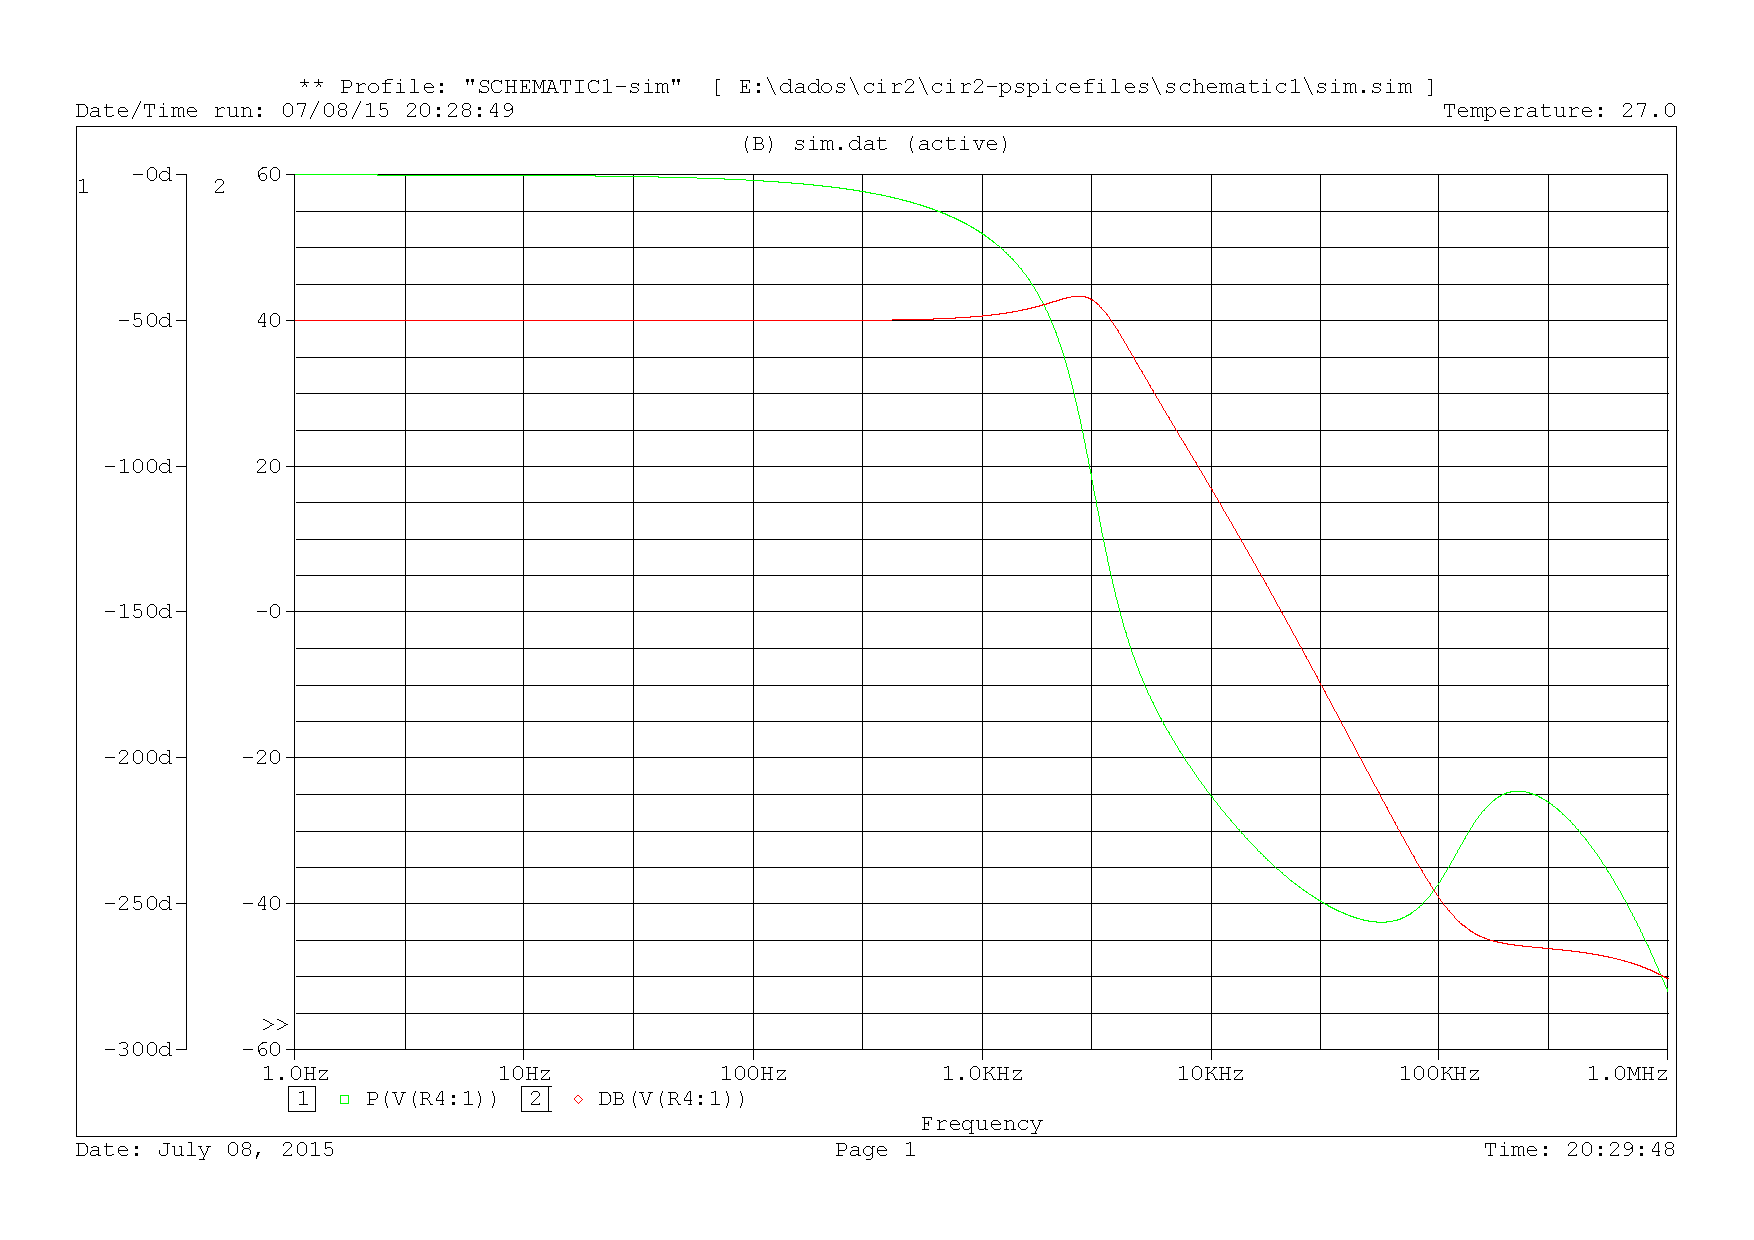
\includegraphics[scale=0.5]{Imagens/bode3.pdf}
\caption{Frequência e fase para segundo estágio do filtro em cascata.}
\label{f_bode3}
\end{figure}

A saída do amplificador em cascata é exibida na figura \ref{f_bode4}, onde foi encontrado que a frequência de corte é de $f_{c1} = 2735 \quad [Hz]$. O filtro possui resposta em frequência do tipo passa baixas de ordem quatro, com atenuação de -22dB/oitava.

\begin{figure}[H]
\centering
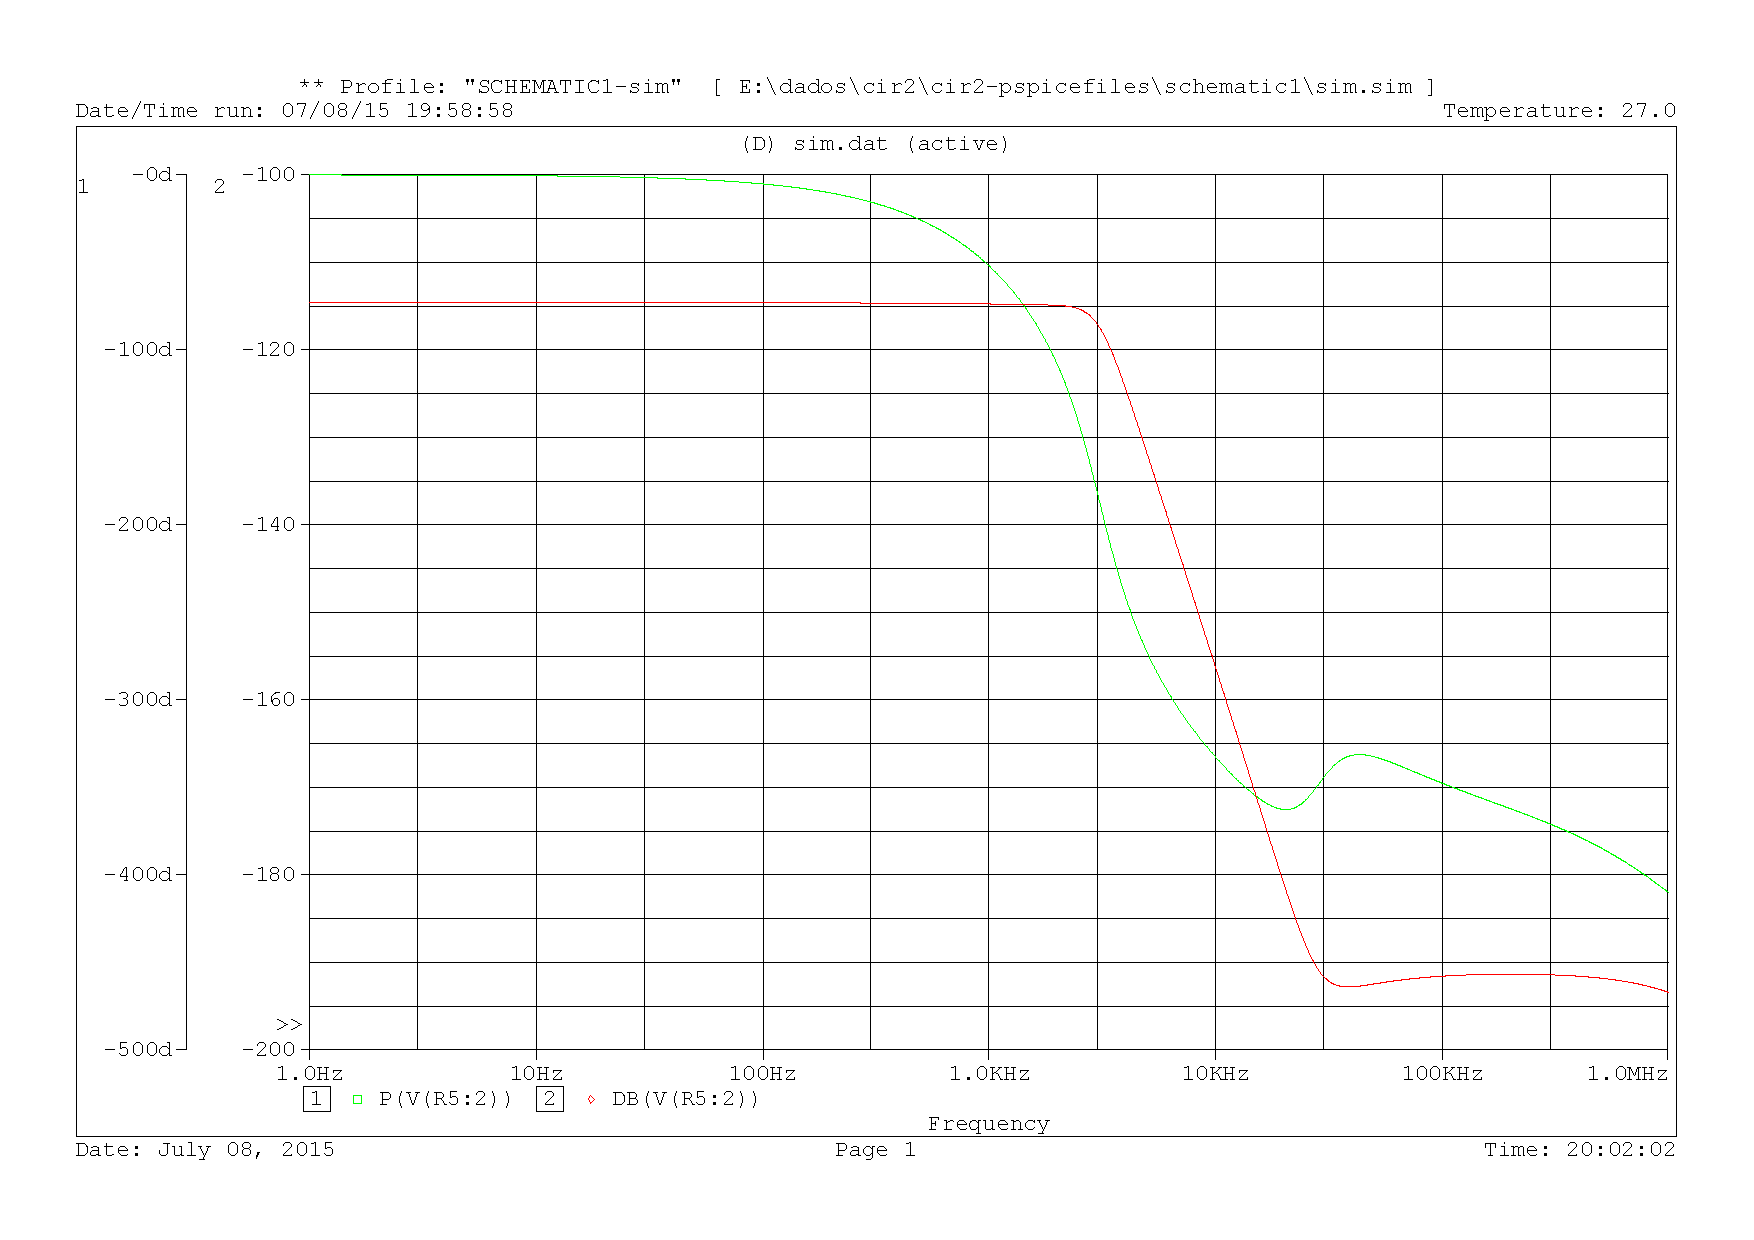
\includegraphics[scale=0.5]{Imagens/bode4.pdf}
\caption{Frequência e fase para primeiro estágio do filtro em cascata.}
\label{f_bode4}
\end{figure}

Para a ultima etapa, foi inserido um sinal de onda quadrada com frequência de 2461 Hz na entrada do filtro em cascata. A onda encontrada na saída está na figura \ref{f_square}.

\begin{figure}[H]
\centering
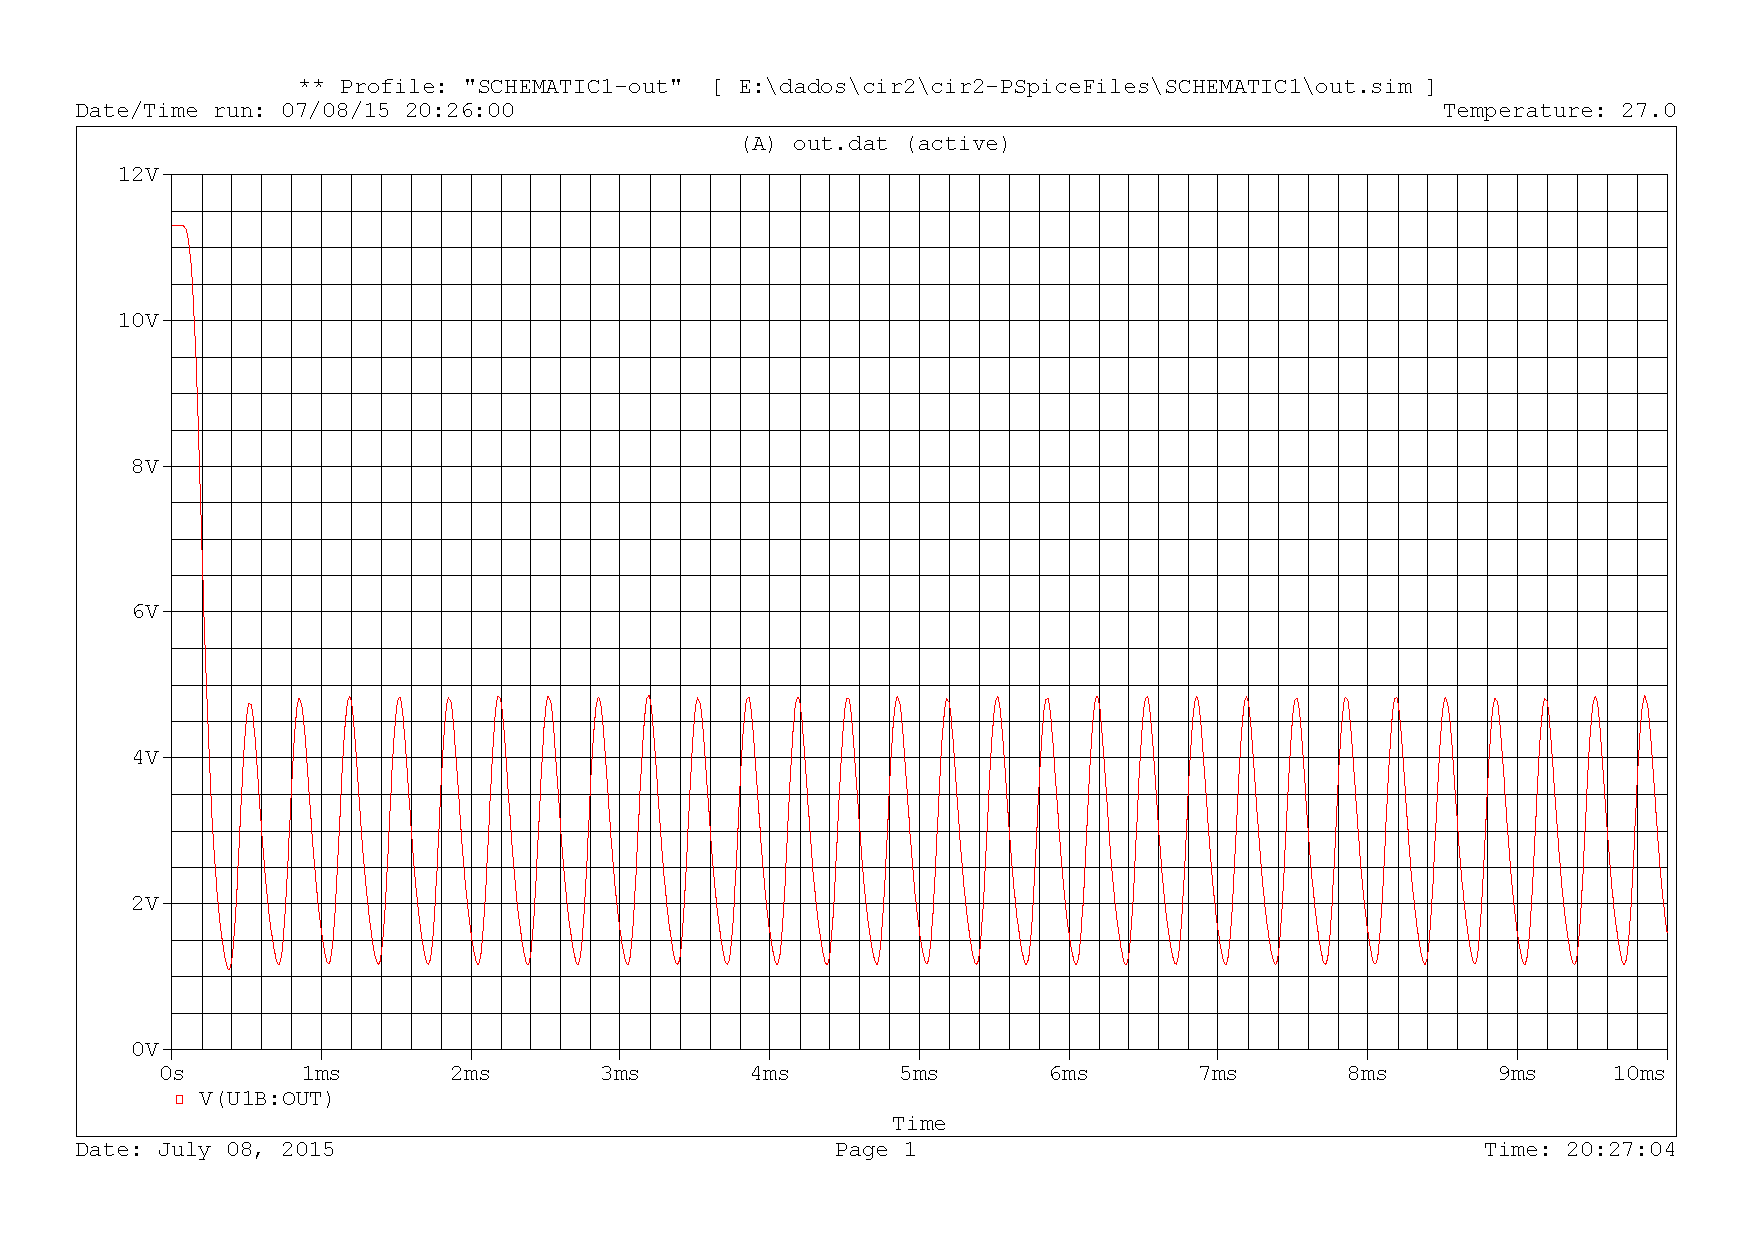
\includegraphics[scale=0.5]{Imagens/square.pdf}
\caption{Frequência e fase para primeiro estágio do filtro em cascata.}
\label{f_square}
\end{figure}
